\begin{figure}[tbp]
\centering
\begin{singlespace}
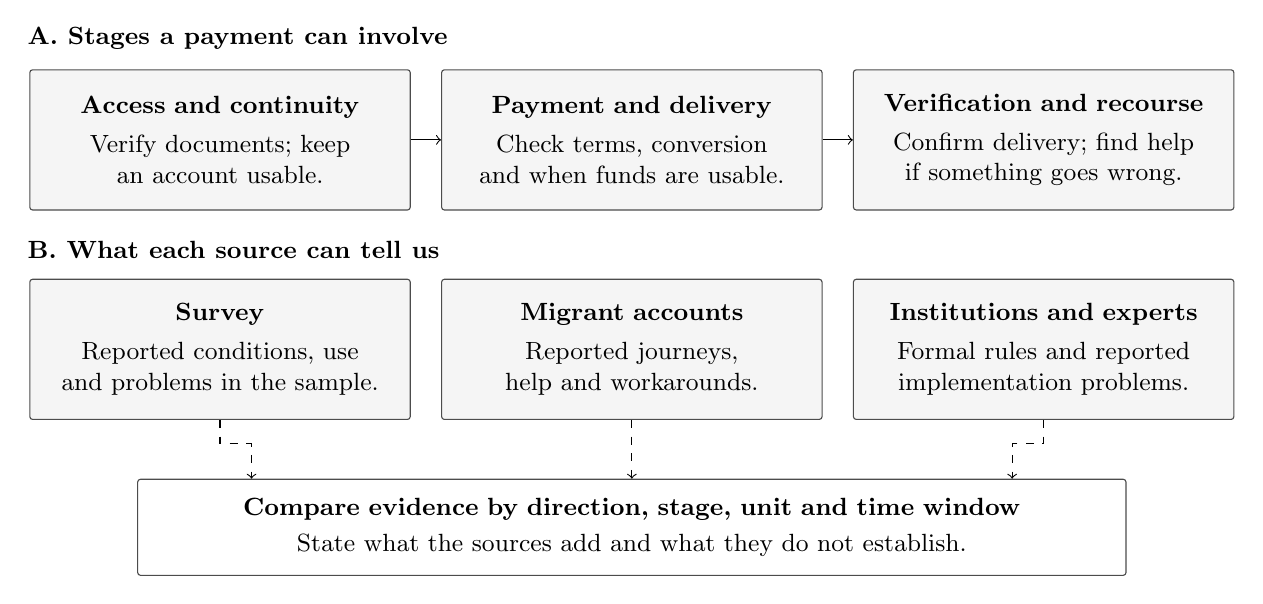
\begin{tikzpicture}[
  font=\small,
  card/.style={draw=black!70, fill=black!4, rounded corners=1pt, anchor=north,
    text width=4.48cm, align=center, inner xsep=5pt, inner ysep=4pt, minimum height=1.78cm},
  heading/.style={font=\small\bfseries, anchor=south west, inner sep=0pt}
]
  \node[heading] at (-7.68,0.24) {A. Stages a payment can involve};
  \node[card] (access) at (-5.23,0) {\textbf{Access and continuity}\\[3pt]
    Verify documents; keep\\an account usable.};
  \node[card] (delivery) at (0,0) {\textbf{Payment and delivery}\\[3pt]
    Check terms, conversion\\and when funds are usable.};
  \node[card] (remedy) at (5.23,0) {\textbf{Verification and recourse}\\[3pt]
    Confirm delivery; find help\\if something goes wrong.};
  \draw[->] (access.east) -- (delivery.west);
  \draw[->] (delivery.east) -- (remedy.west);

  \node[heading] at (-7.68,-2.41) {B. What each source can tell us};
  \node[card] (survey) at (-5.23,-2.66) {\textbf{Survey}\\[3pt]
    Reported conditions, use\\and problems in the sample.};
  \node[card] (migrants) at (0,-2.66) {\textbf{Migrant accounts}\\[3pt]
    Reported journeys,\\help and workarounds.};
  \node[card] (institutions) at (5.23,-2.66) {\textbf{Institutions and experts}\\[3pt]
    Formal rules and reported\\implementation problems.};
  \node[card,text width=12.2cm,minimum height=1.22cm,fill=white] (joint) at (0,-5.20)
    {\textbf{Compare evidence by direction, stage, unit and time window}\\[2pt]
     State what the sources add and what they do not establish.};
  \draw[dashed,->] (survey.south) -- ++(0,-0.30) -| ([xshift=-4.83cm]joint.north);
  \draw[dashed,->] (migrants.south) -- (joint.north);
  \draw[dashed,->] (institutions.south) -- ++(0,-0.30) -| ([xshift=4.83cm]joint.north);
\end{tikzpicture}
\end{singlespace}
\caption{A payment pathway and how the study compares evidence}
\label{fig:payment-evidence-map}
\begin{minipage}{0.94\linewidth}
\smallskip\footnotesize\raggedright
Notes: Solid arrows organize possible stages of a payment. They are not causal links or a required sequence. Dashed arrows show where the strands meet for interpretation, not matching of individuals or transactions. A documented rule, an account of how a transaction unfolds and a survey frequency support different claims.\par
Source: Authors' framework and evidence integration procedure.
\end{minipage}
\end{figure}
